\subsection{CAMARA \acsp{API} Integration}
\label{chap:proposal:exposure:camara}

Network application developers who wish to incorporate adaptive network behavior into their applications must interact with the network through the \acs{NEF} northbound \acsp{API} described in Section~\ref{chap:proposal:exposure:nef}. This can be accomplished in one of the following ways: (i) interacting directly with the \acs{NEF} northbound \acsp{API}, which requires familiarity with the \acs{3GPP} ecosystem, specifications and data models, imposing a significant burden on developers lacking the necessary telco expertise; or (ii) interacting with the network through CAMARA \acsp{API}, which abstract the complexity and underlying interactions with the \acs{NEF} and any other components contributing to the offered service, through a user-friendly interface.

The CAMARA initiative focuses on standardizing \acsp{API} at the northbound of the network, defining what capabilities are exposed and how application developers can interact with them to easily integrate network behavior into their applications. However, the southbound realization of those northbound \acsp{API}, i.e. their internal implementation, is deliberately left to each network operator. Nevertheless, \acs{GSMA} produces guideline documents, such as \textit{\acs{NBI} \acsp{API} Realisation in the \acs{SBI}}~\cite{gsmaNbiRealization}, describing how CAMARA \acs{API} operations can be realized through the \acsp{API} and procedures available in the operator's network, including via \acs{NEF} northbound interfaces.

The CAMARA \acsp{API} integration proposed in this section is derived from this reference realization model, mapping CAMARA operations to the corresponding \acs{NEF} interactions. Under this model, each CAMARA \acs{API} considered in the testbed has a counterpart among the \acs{NEF} northbound \acsp{API}, exposing a simplified view over the same network capability. However, not all CAMARA \acsp{API} map directly to \acs{NEF} interfaces, as some provide auxiliary functionality within the CAMARA ecosystem, such as the \textit{Application Profiles} \acs{API}. Table~\ref{tab:proposal:exposure:camara:nef_mapping} presents the \acs{NEF} and CAMARA \acsp{API} considered for the testbed, organized by the network capabilities they expose and accompanied by representative vertical use cases.

\begin{table}[htbp]
    \centering
    \renewcommand\tabularxcolumn[1]{m{#1}}
    \begin{tabularx}{\textwidth}{|
        >{\RaggedRight\arraybackslash}m{\widthof{\acs{QoS} control}}|
        >{\RaggedRight\arraybackslash}m{\widthof{\textit{AsSessionWithQoS}}}|
        >{\RaggedRight\arraybackslash}m{\widthof{Device Reachability Status,}}|
        >{\RaggedRight\arraybackslash}X|}
        \hline
        \textbf{Capability} & \textbf{\acs{NEF} \acs{API}} & \textbf{CAMARA \acs{API}} & \textbf{Use Cases} \\
        \hline
        \acs{QoS} control & \textit{AsSessionWithQoS} & \acs{QoD} & \acs{QoS} guarantees in \acs{PPDR}, eHealth,\newline live broadcasting \\
        \hline
        \acs{UE} event monitoring & \textit{MonitoringEvent} & Device Location,\newline Device Reachability Status,\newline Device Roaming Status & Geofencing,\newline fleet tracking,\newline detection of unreachable or roaming devices \\
        \hline
        Network analytics & \textit{AnalyticsExposure} & Application Profiles,\newline Connectivity Insights Subscriptions & Bitrate adaptation in video streaming,\newline detection of degraded network conditions \\
        \hline
    \end{tabularx}
    \caption{Correspondence between \acs{NEF} and CAMARA \acsp{API}}
    \label{tab:proposal:exposure:camara:nef_mapping}
\end{table}


Among these, the following subsections detail the proposed \acs{NBI} realization procedure for the \textit{Application Profiles} and \textit{Connectivity Insights Subscriptions} CAMARA \acsp{API}, which will be subject to implementation in the following chapter.

\subsubsection{Application Profiles \acs{API}}
\label{chap:proposal:exposure:camara:profiles}

The \textit{Application Profiles} \acs{API} enables network application developers to share essential information about their applications with the network and other CAMARA \acsp{API}, informing their behavior and decisions~\cite{CAMARAApplicationProfiles}. The \acs{API} focuses on defining network quality thresholds and compute resource requirements needed by the application, which naturally translate into a broad range of use cases. Across media streaming, online gaming, and video conferencing, services can benefit from the use of such an \acs{API} to verify network conditions (e.g. bandwidth, latency, jitter, packet loss) against the desired requirements and dynamically adapt their behavior accordingly. The same profile may also assist network operators in allocating resources and defining \acsp{SLA}, based on the application’s defined needs.

Figure~\ref{fig:flow:CAMARAapplicationProfiles} illustrates the \acs{NBI} realization for the \textit{Application Profiles} \acs{API}, as defined in the \acs{GSMA} reference model~\cite{gsmaNbiRealization}. Under this model, the CAMARA \acsp{API} are exposed by an Operator Platform, acting as an \acs{AF} encapsulating the \acs{NEF}, which internally defines a series of functional blocks, such as the \acs{NBI} \acs{API} Gateway, i.e. the CAMARA northbound endpoints. The Operator Platform also defines the Application Profile Storage Function, which can be considered as a stateful component (database) for storing created application profiles.

The \acs{API} exposes all the endpoints necessary to perform all \acs{CRUD} operations on an Application Profile~\cite{CAMARAApplicationProfilesRelease}. An Application Profile, expressed by the \texttt{ApplicationProfile} schema, defines application thresholds provided for network quality, including packet delay budget, minimum downstream and 
upstream rates, packet error loss rate and jitter, as well as compute resource requirements, such as target min \acs{CPU}, memory and \acs{GPU} specification.

\begin{figure}[htpb]
    \centering
    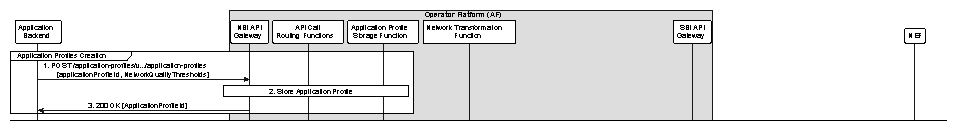
\includegraphics[width=1\linewidth]{figs/gsma-application-profiles.pdf}
    \caption{\acs{NBI} Realization for Application Profiles \acs{API}~\cite{gsmaNbiRealization}}
    \label{fig:flow:CAMARAapplicationProfiles}
\end{figure}

The sequence diagram focuses on the application profiles creation procedure. The application backend, e.g. a network application, submits a POST request to the CAMARA \acs{API} endpoint specifying the profile application requirements through the \texttt{Application\allowbreak Profile\allowbreak Request} record~\cite{CAMARAApplicationProfilesRelease}. On success, CAMARA stores the profile on the local storage repository and returns the created resource identified by a unique profile identifier. This identifier will subsequently be referenced/used in all further \acs{API} operations (retrieval, update and deletion), or by any other CAMARA \acsp{API} that consume the profile.

Throughout this workflow, there is no interaction with the \acs{NEF} or the \acs{5GC}, showcased by the absence of requests to the Network Transformation Function (i.e. the CAMARA translation layer) and the \acs{SBI} \acs{API} Gateway. This emphasizes the role of the \textit{Application Profiles} \acs{API} as a management interface over a shared profile repository, storing requirement declarations that other CAMARA \acsp{API} and network systems may reference/use to make their own decisions, as is the case of the \textit{Connectivity Insights Subscriptions} \acs{API}, discussed in the following section.

\subsubsection{Connectivity Insights Subscriptions \acs{API}}
\label{chap:proposal:exposure:camara:insights}

The \textit{Connectivity Insights Subscriptions} \acs{API} allows developers to receive continuous updates about network quality through event notifications~\cite{CAMARAConnectivityInsightsSubscriptions}. More specifically, applications can leverage this \acs{API} to monitor network conditions in real-time, receiving alerts when quality metrics fall outside the thresholds defined in their application profile, declared via the CAMARA \textit{Application Profiles} \acs{API}. Therefore, this \acs{API} represents the actual mechanism that makes the use cases specified in the previous section possible. Services which previously used profiles to declare their throughput thresholds, can now subscribe to receive notifications the moment those thresholds are breached, allowing them to take adaptive/proactive measures and prevent service disruption.

Figure~\ref{fig:flow:CAMARAconnectivityInsightsSubscriptions} illustrates the \acs{NBI} realization for the \textit{Connectivity Insights Subscriptions} \acs{API} from the \acs{GSMA} document~\cite{gsmaNbiRealization}. The procedure assumes that an application profile is previously created, as described in Section~\ref{chap:proposal:exposure:camara:profiles} (steps 1 to 3). The application then requests the creation of the analytics subscription, specifying the target device and the application server between which monitoring takes place, along with the callback endpoint (\texttt{sink}) and the referenced application profile. The application profile thus defines the network requirements to be monitored. This establishes a direct dependency between the \textit{Connectivity Insights Subscriptions} \acs{API} and the \textit{Application Profiles} \acs{API}, as a subscription requires a previously created application profile to define the criteria against which observed network conditions are evaluated.

\begin{figure}[htpb]
    \centering
    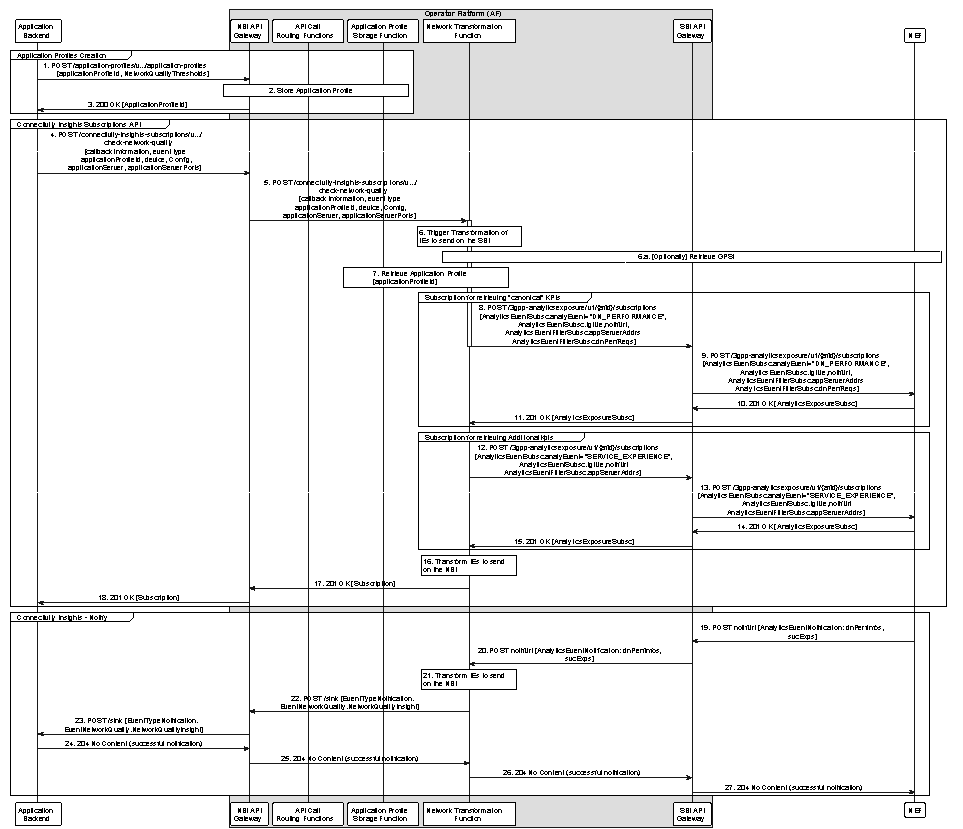
\includegraphics[width=1\linewidth]{figs/gsma-connectivity-insights-subscriptions.pdf}
    \caption{\acs{NBI} Realization for Connectivity Insights Subscriptions \acs{API}~\cite{gsmaNbiRealization}}
    \label{fig:flow:CAMARAconnectivityInsightsSubscriptions}
\end{figure}

Unlike the \textit{Application Profiles} \acs{API}, which involves no interaction with the \acs{NEF} and, consequently, no translation between the CAMARA data models and the underlying \acs{NEF} \acs{3GPP} procedures, the \textit{Connectivity Insights Subscriptions} \acs{API} encapsulates the \acs{NEF} \textit{AnalyticsExposure}~\acs{API}. After receiving the request, the CAMARA layer fetches the application profile from the datastore. The request and the retrieved profile (step 7) are then translated into one or multiple \textit{AnalyticsExposure} subscriptions, which are sent to the \acs{NEF}. The fields of the request are converted into the subscription, passing the device as the target \acs{UE} (\texttt{tgtUe}) and the addressed application server. When the device is identified by its \acs{IP} address, its \acs{GPSI} may first be retrieved from the network (step 6.a). The notification destination of each subscription (\texttt{notifUri}) is also set to the \acs{URI} of the CAMARA service, so that \acs{NEF} notifications are received by the translation layer, before being forwarded to the client. In addition, the network quality thresholds of the application profile are mapped into the reporting thresholds of the \texttt{dnPerfReqs} attribute (for the \texttt{DN\_PERFORMANCE} event), so that the \acs{NEF} notifies the Operator Platform whenever the observed performance crosses them. The reporting requirements of the subscription are, in turn, mapped into the \texttt{analyRepInfo} attribute.

The \acs{NEF} \textit{AnalyticsExposure} \acs{API} supports a wide range of analytics events, covering aspects such as network performance, \acs{UE} communication patterns and service experience~\cite{ETSI_TS_129_522_V18_11_0}. Among these, the \acs{GSMA} reference document selects two events to fulfill the analytics requirements of the \textit{Connectivity Insights Subscriptions} \acs{API}. The \texttt{DN\allowbreak\_PERFORMANCE} event is recommended to retrieve the canonical \acsp{KPI} of the application profile, i.e. the packet delay budget, the downstream and upstream rates, the packet error loss rate and the jitter. A complementary subscription for the \texttt{SERVICE\allowbreak\_EXPERIENCE} event may additionally be created to retrieve additional \acsp{KPI}, namely an indication of the radio conditions and access technology of the device, without any threshold attached.

Once the \textit{AnalyticsExposure} subscriptions are created, the reference to the CAMARA subscription is returned to the application backend. From this point forward, the communication between the involved entities, i.e. application, CAMARA and \acs{NEF}, is entirely based on callbacks. When the notification criteria are met, the \acs{NEF} sends a notification to the \texttt{notifUri} carrying the reported analytics. The CAMARA service then processes these analytics into a network quality insight, indicating, for each threshold of the application profile, if the network meets or is unable the application requirements. At the end, a second callback delivers this insight to the original \texttt{sink} specified by the application in the CAMARA subscription request.

Combined, the \textit{Application Profiles} and \textit{Connectivity Insights Subscriptions} \acsp{API} would allow a network application to declare its network requirements once and be notified whenever the network fails to meet them. The selection of analytics events, the translation into \acs{3GPP} data models and the evaluation of the reported metrics would  be completely abstracted from the consumer, allowing developers without telco expertise to incorporate network analytics into their applications.
